% Options for packages loaded elsewhere
\PassOptionsToPackage{unicode}{hyperref}
\PassOptionsToPackage{hyphens}{url}
%
\documentclass[
  11pt,
]{article}
\usepackage{lmodern}
\usepackage{amssymb,amsmath}
\usepackage{ifxetex,ifluatex}
\ifnum 0\ifxetex 1\fi\ifluatex 1\fi=0 % if pdftex
  \usepackage[T1]{fontenc}
  \usepackage[utf8]{inputenc}
  \usepackage{textcomp} % provide euro and other symbols
\else % if luatex or xetex
  \usepackage{unicode-math}
  \defaultfontfeatures{Scale=MatchLowercase}
  \defaultfontfeatures[\rmfamily]{Ligatures=TeX,Scale=1}
\fi
% Use upquote if available, for straight quotes in verbatim environments
\IfFileExists{upquote.sty}{\usepackage{upquote}}{}
\IfFileExists{microtype.sty}{% use microtype if available
  \usepackage[]{microtype}
  \UseMicrotypeSet[protrusion]{basicmath} % disable protrusion for tt fonts
}{}
\makeatletter
\@ifundefined{KOMAClassName}{% if non-KOMA class
  \IfFileExists{parskip.sty}{%
    \usepackage{parskip}
  }{% else
    \setlength{\parindent}{0pt}
    \setlength{\parskip}{6pt plus 2pt minus 1pt}}
}{% if KOMA class
  \KOMAoptions{parskip=half}}
\makeatother
\usepackage{xcolor}
\IfFileExists{xurl.sty}{\usepackage{xurl}}{} % add URL line breaks if available
\IfFileExists{bookmark.sty}{\usepackage{bookmark}}{\usepackage{hyperref}}
\hypersetup{
  pdftitle={Cross-Structural Research Map, v001},
  pdfauthor={UNNS Research Collective},
  hidelinks,
  pdfcreator={LaTeX via pandoc}}
\urlstyle{same} % disable monospaced font for URLs
\usepackage[margin=25mm]{geometry}
\usepackage{longtable,booktabs}
% Correct order of tables after \paragraph or \subparagraph
\usepackage{etoolbox}
\makeatletter
\patchcmd\longtable{\par}{\if@noskipsec\mbox{}\fi\par}{}{}
\makeatother
% Allow footnotes in longtable head/foot
\IfFileExists{footnotehyper.sty}{\usepackage{footnotehyper}}{\usepackage{footnote}}
\makesavenoteenv{longtable}
\setlength{\emergencystretch}{3em} % prevent overfull lines
\providecommand{\tightlist}{%
  \setlength{\itemsep}{0pt}\setlength{\parskip}{0pt}}
\setcounter{secnumdepth}{-\maxdimen} % remove section numbering
\usepackage{tikz}

\title{Cross-Structural Research Map, v001}
\usepackage{etoolbox}
\makeatletter
\providecommand{\subtitle}[1]{% add subtitle to \maketitle
  \apptocmd{\@title}{\par {\large #1 \par}}{}{}
}
\makeatother
\subtitle{Five connections between the analytic structures and other
branches of the UNNS Substrate}
\author{UNNS Research Collective}
\date{27 November 2026}

\begin{document}
\maketitle

{
\setcounter{tocdepth}{1}
\tableofcontents
}
\hypertarget{scope-and-standing}{%
\section{Scope and standing}\label{scope-and-standing}}

The map takes the five connections of the proposal of 27 November 2026
(\texttt{PROPOSAL\_2026-11-27.md}), identifies source results, states
the common object, proves what can be proved directly and records the
limits. Statements labelled \textbf{M} are derived in this document.
They carry no UNNS Research Collective review and no literature novelty
review. Each connection stops at the level stated here.

Standing labels: \textbf{Exact identity} (the same object or law occurs
in two investigations); \textbf{Proved correspondence} (an established
mathematical map connects them); \textbf{Shared mechanism};
\textbf{Structural analogy}; \textbf{Open connection}.

\begin{longtable}[]{@{}lll@{}}
\toprule
\begin{minipage}[b]{0.14\columnwidth}\raggedright
ID\strut
\end{minipage} & \begin{minipage}[b]{0.34\columnwidth}\raggedright
Connection\strut
\end{minipage} & \begin{minipage}[b]{0.43\columnwidth}\raggedright
Standing reached\strut
\end{minipage}\tabularnewline
\midrule
\endhead
\begin{minipage}[t]{0.14\columnwidth}\raggedright
CSM-01\strut
\end{minipage} & \begin{minipage}[t]{0.34\columnwidth}\raggedright
Composition and history functions\strut
\end{minipage} & \begin{minipage}[t]{0.43\columnwidth}\raggedright
Exact identity (definitional grouping)\strut
\end{minipage}\tabularnewline
\begin{minipage}[t]{0.14\columnwidth}\raggedright
CSM-02\strut
\end{minipage} & \begin{minipage}[t]{0.34\columnwidth}\raggedright
Induced ancestry and correlation functions\strut
\end{minipage} & \begin{minipage}[t]{0.43\columnwidth}\raggedright
Exact identity\strut
\end{minipage}\tabularnewline
\begin{minipage}[t]{0.14\columnwidth}\raggedright
CSM-03\strut
\end{minipage} & \begin{minipage}[t]{0.34\columnwidth}\raggedright
Information geometry and weighted entropy\strut
\end{minipage} & \begin{minipage}[t]{0.43\columnwidth}\raggedright
Proved correspondence for the fibres of words ending at a state\strut
\end{minipage}\tabularnewline
\begin{minipage}[t]{0.14\columnwidth}\raggedright
CSM-04\strut
\end{minipage} & \begin{minipage}[t]{0.34\columnwidth}\raggedright
Generative topology and analytic functions\strut
\end{minipage} & \begin{minipage}[t]{0.43\columnwidth}\raggedright
Proved correspondence at fixed depth; continuation open\strut
\end{minipage}\tabularnewline
\begin{minipage}[t]{0.14\columnwidth}\raggedright
CSM-05\strut
\end{minipage} & \begin{minipage}[t]{0.34\columnwidth}\raggedright
Alternative grammars\strut
\end{minipage} & \begin{minipage}[t]{0.43\columnwidth}\raggedright
Partial classification\strut
\end{minipage}\tabularnewline
\bottomrule
\end{longtable}

Sources outside this collection are in the repository
\texttt{ukbbi/UNNS}, read at commit \texttt{9a1e94c}, and in the local
monograph \emph{Induced Structures in the UNNS Substrate}.

\hypertarget{the-common-object}{%
\section{0. The common object}\label{the-common-object}}

A \emph{grammar} here is a family of labelled maps
\(x\mapsto (p_b/q_b)x\), \(\gcd(p_b,q_b)=1\), admissible when
\(q_b\mid x\), such that only finitely many words end at any given
integer (the integral-image sector with finiteness). By ANS-T03 every
word \(w\) has a minimal source \(K(w)\) and a least endpoint
\(E(w)=K(w)Q(w)\), and the words ending at \(x\) form
\[W(x)=\{w:\ E(w)\mid x\}.\] \(W_k(x)\) is its depth-\(k\) part,
\(H_k(x)=|W_k(x)|\), and \(a_k(n)=\#\{|w|=k: E(w)=n\}\), so that
\(G_k(s)=\sum_na_k(n)n^{-s}\).

The common object of this map is the \textbf{threshold map} \(E\) from
the population of words to the integers ordered by divisibility. It is
the incidence relation \(B(x,w)=1\) if \(E(w)\mid x\).

\begin{center}
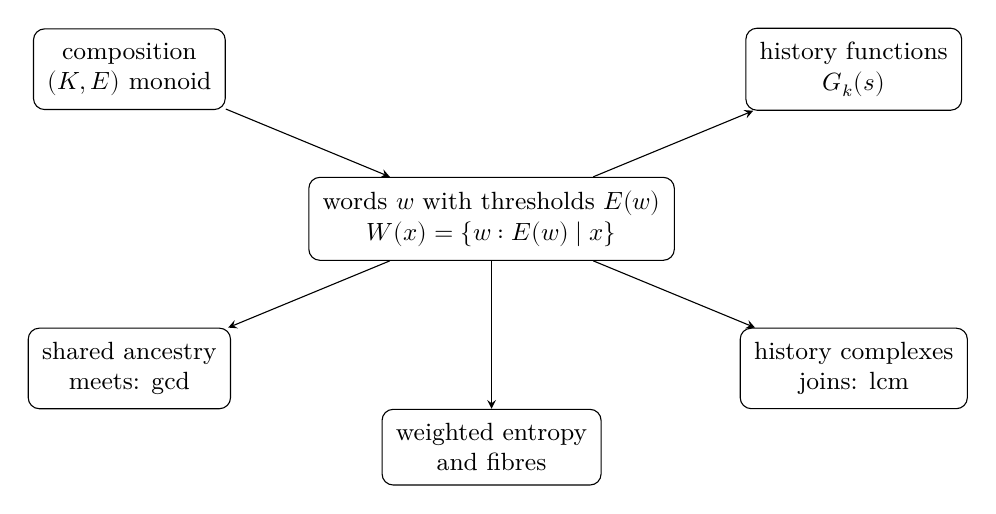
\begin{tikzpicture}[>=stealth,every node/.style={draw,rounded corners,align=center,font=\small,inner sep=5pt}]
\node (E) at (0,0) {words $w$ with thresholds $E(w)$\\ $W(x)=\{w: E(w)\mid x\}$};
\node (A) at (-4.6,1.9) {composition\\ $(K,E)$ monoid};
\node (B) at (4.6,1.9) {history functions\\ $G_k(s)$};
\node (C) at (-4.6,-1.9) {shared ancestry\\ meets: $\gcd$};
\node (D) at (4.6,-1.9) {history complexes\\ joins: $\mathrm{lcm}$};
\node (F) at (0,-2.9) {weighted entropy\\ and fibres};
\draw[->] (A)--(E); \draw[->] (E)--(B); \draw[->] (E)--(C); \draw[->] (E)--(D); \draw[->] (E)--(F);
\end{tikzpicture}
\end{center}

\hypertarget{csm-01.-composition-and-history-functions}{%
\section{CSM-01. Composition and history
functions}\label{csm-01.-composition-and-history-functions}}

\textbf{Sources.} ANS-T04, ANS-T47, ANS-T14. Prime valuation coordinates
\(\mathbb Q_{>0}\cong\bigoplus_p\mathbb Z\) also occur in
\emph{Algebraic and Topological Extensions of the UNNS Generative Law},
v1.1.

\textbf{M1.} The map \(\phi(w)=(K(w),E(w))\) is a homomorphism from
words under concatenation to the pairs with product
\[(K,E)\circ(K',E')=\Big(\frac{KK'}d,\frac{EE'}d\Big),\qquad d=\gcd(E,K').\]
Put \(X=\sum_b\phi(b)\) in the (completed) monoid algebra and
\(m_k(a,b)=\#\{|w|=k:\phi(w)=(a,b)\}\). Then
\(X^k=\sum m_k(a,b)\,(a,b)\) and \(G_k(s)=\Lambda_s(X^k)\) for the
linear functional \(\Lambda_s(a,b)=b^{-s}\).

\emph{Proof.} The product is the composition law: \(w=uv\) is admissible
from the sources whose image under \(u\) lies in both \(E(u)\mathbb Z\)
and \(K(v)\mathbb Z\), that is in
\(\mathrm{lcm}(E(u),K(v))\mathbb Z=(E(u)K(v)/d)\mathbb Z\); dividing by
\(Q(u)\) and multiplying by \(Q(v)\) gives \(K(uv)\) and \(E(uv)\). The
rest is grouping words by \(\phi\). \(\square\)

\textbf{Where the analytic difficulty sits.} \(\Lambda_s\) is not
multiplicative: \(\Lambda_s(uv)=d^{\,s}\Lambda_s(u)\Lambda_s(v)\).
Expanding \(d^{\,s}=\sum_{e\mid d}J_s(e)\) gives the block factorization
of ANS-T47. The multiplier weight \((b/a)^{-s}=Q^{-s}\) \emph{is}
multiplicative and gives \(B(s)^k\). The difference between the two
weights is the source factor \(K^{-s}\).

\textbf{Recovery and limits.} \(F(s,u)=\sum_{|w|=k}E^{-s}K^{-u}\)
determines \(m_k\) (uniqueness of Dirichlet series in two variables).
\(G_k=F(\cdot,0)\) keeps only the marginal in \(E\); no formula
recovering \(m_k\) from \(G_k\) is known here. The prime coordinates on
the two sides are the same valuations, so their agreement is not
independent evidence for a further structure.

\hypertarget{csm-02.-induced-ancestry-and-correlation-functions}{%
\section{CSM-02. Induced ancestry and correlation
functions}\label{csm-02.-induced-ancestry-and-correlation-functions}}

\textbf{Sources.} The meet law \(W(x)\cap W(y)=W(\gcd(x,y))\) is FUG3-T2
and SIB-I SCG-01. The Gram (incidence) form of the overlap kernel is
SCG-09 and the monograph chapter \emph{Overlap Kernels and Induced
Relational Geometry}, whose endpoint decomposition \(\nu=\mu*|W|\) is
the all-depth case of the inversion in ANS-T01 and ANS-T02. The two
lines of work therefore contain the same identity. The monograph kernel
counts non-empty words of all depths; here depth is kept.

\textbf{M2 (transform of shared ancestry).} Let \(r\ge1\) and
\(C_k^{(r)}(x_1,\dots,x_r)=|W_k(x_1)\cap\dots\cap W_k(x_r)|\). Then
\(C_k^{(r)}=H_k(\gcd(x_1,\dots,x_r))\) and, when words of length \(k\)
exist,
\[\sum_{x_1,\dots,x_r\ge1}\frac{C_k^{(r)}(x_1,\dots,x_r)}{x_1^{s_1}\cdots x_r^{s_r}}=\zeta(s_1)\cdots\zeta(s_r)\,G_k(s_1+\dots+s_r),\]
absolutely convergent exactly when every \(\operatorname{Re}s_i>1\) (for
the nesting grammar and \(k\ge0\)).

\emph{Proof.} A word is counted at \((x_1,\dots,x_r)\) exactly when
\(E(w)\) divides every \(x_i\). Sum over \(x_i=E(w)m_i\); the terms are
non-negative at real \(s_i\), giving \(\prod_i\zeta(s_i)E(w)^{-s_i}\).
For \(r\ge1\) and all \(s_i>1\) the argument of \(G_k\) exceeds \(1/2\)
(ANS-T12); if some \(s_i\le1\) the sum over \(m_i\) diverges.
\(\square\)

The case \(r=1\) is ANS-T01 and \(r=2\) is the proposed identity: one
statement covers both. For all depths, \(\sum_kt^kC_k^{(2)}\) transforms
to \(\zeta(s)\zeta(u)\,\mathcal G(s+u,t)\); at \(t=1\) and
\(\operatorname{Re}s,\operatorname{Re}u>1\) one has
\(\operatorname{Re}(s+u)>2>\sigma_c\), so it converges.

\textbf{M3 (rank of the ancestry matrix).} For
\(M_n=[H_k(\gcd(i,j))]_{i,j\le n}\) one has
\(M_n=Z\,\mathrm{diag}(a_k(1),\dots,a_k(n))\,Z^{\mathsf T}\) with
\(Z_{im}=1\) if \(m\mid i\). Hence \(M_n\) is positive semidefinite and
its rank is the number of \(m\le n\) with \(a_k(m)>0\). For the nesting
grammar and \(k\ge1\), \(a_k(1)=0\), so \(M_n\) is singular.
\emph{Proof.} \(H_k(g)=\sum_{m\mid g}a_k(m)\) and \(Z\) is unit
triangular. \(\square\) This is the classical factorization of
greatest-common-divisor matrices (Smith).

\textbf{Limits.} M2 holds in every grammar of the sector for which the
series converge, including the repetition grammar of SCG-08. It
re-expresses \(G_k\) and adds no information about the grammar beyond
\(G_k\).

\hypertarget{csm-03.-information-geometry-and-weighted-entropy}{%
\section{CSM-03. Information geometry and weighted
entropy}\label{csm-03.-information-geometry-and-weighted-entropy}}

\textbf{Sources.} GIG-I: GIG-T1 to GIG-T5 (fibres, uniform-history
entropy). ANS-T12, T48, T49, T50.

For real \(s>1/2\) put \(P_{k,s}(w)=E(w)^{-s}/G_k(s)\). Its entropy is
\(\mathcal H_k(s)=\log G_k(s)-s\,(\log G_k)'(s)\), and
\((\log G_k)''(s)=\mathrm{Var}_{k,s}(\log E)\). These are the standard
partition-function identities. Natural logarithms are used; GIG-I uses
base two.

\textbf{M4 (relation to fibre entropy).} Let \(\sigma>1\) and give pairs
(endpoint \(n\), word \(w\in W_k(n)\)) the probability
\(n^{-\sigma}/(\zeta(\sigma)G_k(\sigma))\). Then (i) the word has law
\(P_{k,\sigma}\); (ii) given the endpoint, the word is uniform on
\(W_k(n)\); (iii) \(N=E(W)\,Z\), where \(Z\) has the zeta law
\(z^{-\sigma}/\zeta(\sigma)\) and is independent of \(W\). Consequently
\[\mathcal H_k(\sigma)+H(Z)=H(N)+\mathbb E\big[\log H_k(N)\big].\]

\emph{Proof.} Summing over \(n=E(w)z\) gives
\(\zeta(\sigma)E(w)^{-\sigma}\), hence (i) and (iii); (ii) holds because
the weight does not depend on \(w\). Compute the joint entropy in both
orders. \(\square\)

So the global weighted entropy equals the entropy of the endpoint, plus
the mean uniform-history entropy of its fibre, minus the entropy of the
free source factor.

\textbf{M5 (complete histories).} GIG-I fibres of complete histories use
squarefree sources, a different fibre from \(W_k(t)\). For the nesting
grammar, if \(F_{k}(t)\) is the set of depth-\(k\) histories ending at
\(t\) from a squarefree source, then for \(\operatorname{Re}s>1\)
\[\sum_{t\ge1}\frac{|F_k(t)|}{t^s}=\frac{\zeta(s)}{\zeta(2s)}\sum_{\substack{|w|=k\\K(w)\ \mathrm{squarefree}}}E(w)^{-s}\prod_{p\mid K(w)}(1+p^{-s})^{-1}.\]

\emph{Proof.} The sources of \(w\) are \(K(w)m\), ending at \(E(w)m\).
\(K(w)m\) is squarefree exactly when \(K(w)\) and \(m\) are squarefree
and coprime, and \(\sum m^{-s}\) over such \(m\) is
\(\prod_{p\nmid K}(1+p^{-s})\). \(\square\) Complete histories therefore
correspond to a \emph{source-restricted} history function, not to
\(\zeta G_k\).

\textbf{M6 (order of the entropy at \(s=1\)).} Let \(L=\log k\) and
\(\mu_k=\mathbb E_{k,1}[\log E]\). Then
\[0.422\le\liminf_{k\to\infty}\frac{\mu_k}{kL}\le\limsup_{k\to\infty}\frac{\mu_k}{kL}\le1.791,\qquad\mathcal H_k(1)=\mu_k+k\log\log k+O(k).\]
In particular \(\mathcal H_k(1)\) has exact order \(k\log k\).

\emph{Proof.} \(f=\log G_k\) is convex on \(s>1/2\) and
\(\mu_k=-f'(1)\). Hence for \(\tau>0\) and \(h=\tau/L\),
\[\frac{f(1)-f(1+h)}h\le\mu_k\le\frac{f(1-h)-f(1)}h.\] Let
\(c_0=1.10791\) (a lower value for the constant of ANS-T49) and
\(\mathrm{Ein}(\tau)=\int_0^1(1-e^{-\tau u})\,du/u\). By ANS-T49 and
ANS-T50, \(f(1)\ge k(\log L+\log c_0+o(1))\) and
\(f(1\pm h)\le k(\log L+\gamma-\mathrm{Ein}(\pm\tau)+o(1))\). Therefore
\[\frac{\log c_0-\gamma+\mathrm{Ein}(\tau)}{\tau}\le\liminf\frac{\mu_k}{kL},\qquad\limsup\frac{\mu_k}{kL}\le\frac{\gamma-\mathrm{Ein}(-\tau)-\log c_0}{\tau}.\]
Take \(\tau=2.07\) in the first and \(\tau=1.07\) in the second
(numerical evaluation: \(0.42242\) and \(1.79011\)). The entropy formula
is \(\mathcal H_k(1)=f(1)+\mu_k\) with ANS-T48. \(\square\)

The logarithm of the partition function, of order \(k\log\log k\), is
thus of smaller order than the entropy: at \(s=1\) the entropy is
carried by the mean logarithm of the endpoint.

\textbf{Open.} A limit of \(\mu_k/(k\log k)\); concentration of
\(\log E\); a statement like M4 for \(1/2<\sigma\le1\), where the zeta
law does not exist; a relation between \(\mathcal H_k\) and the GIG-I
swap-class decomposition.

\hypertarget{csm-04.-generative-topology-and-analytic-functions}{%
\section{CSM-04. Generative topology and analytic
functions}\label{csm-04.-generative-topology-and-analytic-functions}}

\textbf{Sources.} GIG-I v001 to v007 (permutohedral history complexes,
thresholds of cells, certified homology); GEO-HD-1D.

\textbf{Construction.} Fix \(k\). For a set \(C\) of \(k\) distinct
letters, the cells are the faces of the permutohedron on \(C\) (ordered
partitions of \(C\) into blocks); the vertices of a cell are the words
obtained by ordering within blocks. \(\mathcal K_x\) is the union over
\(C\) of the cells all of whose vertices lie in \(W_k(x)\). Homology is
over \(\mathbb F_2\). Words with repeated letters are not included.

\textbf{M7.} Let \(E(c)=\mathrm{lcm}\{E(v):v\text{ a vertex of }c\}\).

\begin{enumerate}
\def\labelenumi{\arabic{enumi}.}
\tightlist
\item
  \(c\subset\mathcal K_x\) exactly when \(E(c)\mid x\).
\item
  For \(\operatorname{Re}s>1\),
  \[\sum_{x\ge1}\frac{\chi(\mathcal K_x)}{x^s}=\zeta(s)\sum_c\frac{(-1)^{\dim c}}{E(c)^s},\]
  and similarly, without signs, for the number of cells of each
  dimension.
\item
  Every \(\mathcal T_j(s)=\sum_x\beta_j(\mathcal K_x)x^{-s}\) converges
  absolutely for \(\operatorname{Re}s>1\). If one
  \(\beta_j(\mathcal K_{x_0})\) is non-zero, the abscissa of
  \(\mathcal T_j\) is exactly \(1\).
\item
  If \(\beta_{C,j}(x)\) is the contribution of \(C\), it depends only on
  \(\gcd(x,L_C)\), \(L_C=\mathrm{lcm}\) of all \(E(c)\) for \(C\).
  Hence, coefficient by coefficient,
  \(\mathcal T_j(s)=\zeta(s)\sum_C\sum_{d\mid L_C}b_{C,j}(d)\,d^{-s}\)
  with the integers \(b_{C,j}=\mu*\beta_{C,j}\) on the divisors of
  \(L_C\).
\end{enumerate}

\emph{Proof.} (1) is \(W_k(x)=\{E\mid x\}\) applied to all vertices. (2)
Each cell contributes at the multiples of \(E(c)\); since
\(E(c)\ge E(v)\) and a word lies in a bounded number of cells,
\(\sum_cE(c)^{-\sigma}\ll_kG_k(\sigma)<\infty\) for \(\sigma>\frac12\).
(3) \(\beta_j\le\) number of \(j\)-cells, so (2) gives convergence.
Choose \(C\) with \(\beta_{C,j}(x_0)>0\). If \(\gcd(m,L_C)=1\) the cells
of \(C\) present at \(mx_0\) are those present at \(x_0\), so
\(\beta_j(\mathcal K_{mx_0})\ge\beta_{C,j}(x_0)\) on a set of positive
density. (4) By (1) the cells of \(C\) present at \(x\) are determined
by \(\gcd(x,L_C)\); apply Möbius inversion on the divisors of \(L_C\). A
given \(d\) receives contributions from finitely many \(C\), since a
non-empty complex needs a word with \(E\mid d\). \(\square\)

\textbf{A non-zero case.} For \(k=4\), \(C=\{2,3,14,15\}\) and
\(x=1\,382\,400\) (source \(210\), the loop of GIG-T10) the contribution
has \(\beta_0=\beta_1=1\); here \(L_C=8\,294\,400\). Hence
\(\mathcal T_1\) at depth four has abscissa exactly \(1\).

\textbf{Meets and joins.} CSM-02 asks which words two endpoints share:
\(B B^{\mathsf T}\) and a greatest common divisor. Cells ask which
endpoints several words share: for two words
\(\sum_xx^{-s}B(x,u)B(x,v)=\zeta(s)\,\mathrm{lcm}(E(u),E(v))^{-s}\). The
two representations are dual readings of the same incidence relation.

\textbf{Limits.} The Euler characteristic and cell series need only
thresholds of cells; Betti numbers also need boundary ranks, and
\(\mathcal T_j\) has signed coefficients in (4). The cell thresholds are
joint data of several words; no formula expressing them through \(G_k\)
is known here, and GIG-I (GIG-T9) shows that history counts and class
sizes of arithmetic pieces do not determine their homology.
\textbf{Open:} continuation of \(\mathcal T_j\) and of the
Euler-characteristic series to the left of \(1\) (for the cell sum, to
the left of \(\frac12\)); complexes including repeated letters; all
depths together; any analytic signature of the appearance of higher
homology.

\hypertarget{csm-05.-alternative-grammars}{%
\section{CSM-05. Alternative
grammars}\label{csm-05.-alternative-grammars}}

\begin{longtable}[]{@{}lll@{}}
\toprule
\begin{minipage}[b]{0.30\columnwidth}\raggedright
Statement\strut
\end{minipage} & \begin{minipage}[b]{0.40\columnwidth}\raggedright
Holds for\strut
\end{minipage} & \begin{minipage}[b]{0.22\columnwidth}\raggedright
Reference\strut
\end{minipage}\tabularnewline
\midrule
\endhead
\begin{minipage}[t]{0.30\columnwidth}\raggedright
Composition law; \(W(x)=\{E\mid x\}\); meet law\strut
\end{minipage} & \begin{minipage}[t]{0.40\columnwidth}\raggedright
grammars of Section 0\strut
\end{minipage} & \begin{minipage}[t]{0.22\columnwidth}\raggedright
ANS-T03, M1\strut
\end{minipage}\tabularnewline
\begin{minipage}[t]{0.30\columnwidth}\raggedright
Factorization \(\zeta\cdot G\); transform of shared ancestry;
ancestry-matrix rank\strut
\end{minipage} & \begin{minipage}[t]{0.40\columnwidth}\raggedright
the same, where series converge\strut
\end{minipage} & \begin{minipage}[t]{0.22\columnwidth}\raggedright
ANS-T01, M2, M3\strut
\end{minipage}\tabularnewline
\begin{minipage}[t]{0.30\columnwidth}\raggedright
Partition-function identities; M4\strut
\end{minipage} & \begin{minipage}[t]{0.40\columnwidth}\raggedright
the same, where series converge\strut
\end{minipage} & \begin{minipage}[t]{0.22\columnwidth}\raggedright
M4\strut
\end{minipage}\tabularnewline
\begin{minipage}[t]{0.30\columnwidth}\raggedright
Cell transform\strut
\end{minipage} & \begin{minipage}[t]{0.40\columnwidth}\raggedright
the same, for distinct-letter complexes, where \(\sum_cE(c)^{-s}\)
converges\strut
\end{minipage} & \begin{minipage}[t]{0.22\columnwidth}\raggedright
M7\strut
\end{minipage}\tabularnewline
\begin{minipage}[t]{0.30\columnwidth}\raggedright
Rational history function\strut
\end{minipage} & \begin{minipage}[t]{0.40\columnwidth}\raggedright
unit denominators\strut
\end{minipage} & \begin{minipage}[t]{0.22\columnwidth}\raggedright
ANS-T08\strut
\end{minipage}\tabularnewline
\begin{minipage}[t]{0.30\columnwidth}\raggedright
Saturation and growth bound\strut
\end{minipage} & \begin{minipage}[t]{0.40\columnwidth}\raggedright
positive weighted drift\strut
\end{minipage} & \begin{minipage}[t]{0.22\columnwidth}\raggedright
ANS-T11\strut
\end{minipage}\tabularnewline
\begin{minipage}[t]{0.30\columnwidth}\raggedright
Exponent, suppression, drift dichotomy\strut
\end{minipage} & \begin{minipage}[t]{0.40\columnwidth}\raggedright
extended torsion grammars, per class\strut
\end{minipage} & \begin{minipage}[t]{0.22\columnwidth}\raggedright
ANS2-T16\strut
\end{minipage}\tabularnewline
\begin{minipage}[t]{0.30\columnwidth}\raggedright
\(\sigma_c=1.5463810\ldots\); \(1+z^2+z^3\); natural boundary of
\(G_2\); growth at \(s=1\)\strut
\end{minipage} & \begin{minipage}[t]{0.40\columnwidth}\raggedright
nesting grammar\strut
\end{minipage} & \begin{minipage}[t]{0.22\columnwidth}\raggedright
T09, T45a, T48\strut
\end{minipage}\tabularnewline
\bottomrule
\end{longtable}

\textbf{M8.} If every \(q_b=1\), then \(E(w)=Q(w)\) is independent of
the order of letters, so for each \(C\) the complex at \(x\) is empty or
the whole permutohedron. Hence \(\beta_j(\mathcal K_x)=0\) for
\(j\ge1\). \(\square\)

Together with ANS-T08: unit denominators give both a rational history
function and trivial history topology. Non-trivial analytic coupling and
non-trivial topology both require denominators. The converse is not
claimed, and no criterion deciding which denominators produce a natural
boundary or non-trivial homology is known here.

\hypertarget{what-the-map-establishes}{%
\section{What the map establishes}\label{what-the-map-establishes}}

\begin{enumerate}
\def\labelenumi{\arabic{enumi}.}
\tightlist
\item
  The five representations of CSM-01 to CSM-04 are functions of one
  incidence relation between states and words. For CSM-02 and CSM-03
  this is a direct transform; for topology it needs the joint thresholds
  of cells.
\item
  Recoverability is uneven. \(a_k\), \(G_k\), \(H_k\) and the kernels
  \(C_k^{(r)}\) determine one another. The pairs \((K,E)\) need a second
  variable. Topology needs the thresholds of cells.
\item
  The identities that connect the branches hold across the sector, so
  they do not distinguish the nesting grammar. The results that do
  distinguish it concern the \emph{distribution} of \(E\) and of its
  joins.
\item
  This answers part of the question why the structures arise together:
  at the level of representation they come from divisibility of one
  threshold. It does not transfer the deep theorems of one branch to
  another.
\end{enumerate}

\hypertarget{open-connections}{%
\section{Open connections}\label{open-connections}}

\begin{longtable}[]{@{}ll@{}}
\toprule
\begin{minipage}[b]{0.64\columnwidth}\raggedright
Candidate\strut
\end{minipage} & \begin{minipage}[b]{0.30\columnwidth}\raggedright
Standing\strut
\end{minipage}\tabularnewline
\midrule
\endhead
\begin{minipage}[t]{0.64\columnwidth}\raggedright
ATL-02 saturation and obstruction with structural survival and common
refinement\strut
\end{minipage} & \begin{minipage}[t]{0.30\columnwidth}\raggedright
Open connection\strut
\end{minipage}\tabularnewline
\begin{minipage}[t]{0.64\columnwidth}\raggedright
ATL-03 and ATL-04 with collective dynamics of the arithmetic-dynamics
studies\strut
\end{minipage} & \begin{minipage}[t]{0.30\columnwidth}\raggedright
Open connection\strut
\end{minipage}\tabularnewline
\begin{minipage}[t]{0.64\columnwidth}\raggedright
Quadratic pole order \(\lfloor k^2/4\rfloor\) with dimension of history
complexes\strut
\end{minipage} & \begin{minipage}[t]{0.30\columnwidth}\raggedright
Structural analogy\strut
\end{minipage}\tabularnewline
\begin{minipage}[t]{0.64\columnwidth}\raggedright
Natural boundary of \(G_2\) with homological obstruction\strut
\end{minipage} & \begin{minipage}[t]{0.30\columnwidth}\raggedright
Structural analogy\strut
\end{minipage}\tabularnewline
\begin{minipage}[t]{0.64\columnwidth}\raggedright
Entropy--admissibility principle (ATL-11) with GIG recovery
results\strut
\end{minipage} & \begin{minipage}[t]{0.30\columnwidth}\raggedright
Open connection\strut
\end{minipage}\tabularnewline
\bottomrule
\end{longtable}

\hypertarget{checks}{%
\section{Checks}\label{checks}}

\texttt{verification/verify\_map.py} tests the composition law, the
fibre description, the meet and coefficient identities, the matrix rank,
the complete-history identity, cell activation, the depth-four example
and the constants of M6 on finite ranges
(\texttt{verification/RESULTS.txt}). Finite checks do not prove the
statements. The repository search for an earlier occurrence of M2 was a
text search of the Markdown and TeX sources, not a literature review.

\end{document}
